\documentclass{article}
\usepackage{amsmath}
\usepackage{graphicx}
\usepackage{amsfonts}
\usepackage{amssymb}
\usepackage{bm}
\usepackage[colorlinks=true, linkcolor=black, urlcolor=blue]{hyperref}
\usepackage{fontspec}
\setmainfont{Times New Roman}
\usepackage{listings}
\usepackage{xcolor}
\usepackage{mathtools}
\usepackage{tcolorbox}
\tcbuselibrary{breakable}
\usepackage{fancyvrb}
\usepackage{placeins}
\usepackage{booktabs}
\usepackage{float}
\usepackage[a4paper, margin=1in]{geometry}
\usepackage{subcaption}
\usepackage{tikz}
\usetikzlibrary{arrows.meta,positioning,fit,backgrounds,calc}
\usepackage{pgfplots}
\pgfplotsset{compat=1.18}
% ---------- COLORS ----------
\definecolor{inputblue}{RGB}{66,165,245}
\definecolor{sigmoidpurple}{RGB}{171,71,188}
\definecolor{hidden1}{RGB}{129,199,132}
\definecolor{hidden2}{RGB}{255,193,7}
\definecolor{reluorange}{RGB}{255,167,38}
\definecolor{bncyan}{RGB}{0,188,212}
\definecolor{outputred}{RGB}{244,67,54}
\definecolor{residualgray}{RGB}{96,125,139}

% ---------- TIKZ STYLES ----------
\tikzset{
	>=Latex,
	neuron/.style={
		circle,
		draw,
		thick,
		minimum size=7mm,
		inner sep=0pt
	},
	layerbox/.style={
		draw,
		rounded corners,
		thick,
		inner sep=4pt,
		fill opacity=0.06
	},
	conn/.style={
		-{Latex[length=2mm,width=1.6mm]},
		line width=0.6pt
	}
}


\lstset{
  language=Matlab,
  basicstyle=\small\ttfamily,
  keywordstyle=\color{blue},
  commentstyle=\color{green!70!black},
  stringstyle=\color{red},
  showstringspaces=false,
  frame=single,
  captionpos=b,
  % --- ADD THESE THREE LINES TO FIX LINE BREAKING ---
  breaklines=true,                 % 1. Enables automatic line breaking
  breakatwhitespace=false,         % 2. Allows breaking lines at non-whitespace
  postbreak=\mbox{\textcolor{red}{$\hookrightarrow$}\space} % 3. Adds an arrow to show a line break
}

\begin{document}
\begin{titlepage}
  \centering
  
\includegraphics[width=0.3\textwidth]{download.png} \\[1.5cm]
  {\huge \textbf{K.N. Toosi University}}\\[2cm]
  {\Large \textbf{Aidin Sahneh}}\\[0.5cm] 
  {\large \textbf{\\ Student ID:} 40120243}\\[0.7cm]
  {\Large \textbf{Amir Hosseinpoor}}\\[0.5cm] 
  {\large \textbf{\\ Student ID:} 40117393}\\[0.7cm]
  {\Large \textbf{Hamed Behrouzi Moghaddam}}\\[0.5cm] 
  {\large \textbf{\\ Student ID:} 40215633 }\\[0.7cm]
  {\Large \textbf{\\ Course:} Introduction to MachineLearning}\\[0.3cm]
  {\large \textbf{Instructor:} Dr. Nikoofard}\\[0.5cm]
  
  
 \vfill
 {\large \textbf{Project Source Code:} \href{https://colab.research.google.com/drive/1T095P_2YAXzVvQechae1NYIQ3rLlye0n#scrollTo=58c3isRzrx8e}{Interactive Google Colab Notebook (Question 5)}}
  
  
\end{titlepage}

\newpage
\tableofcontents
\newpage


\section{Question 1: Analysis of Forward / Backward Propagation and Dying ReLUs}

	Consider a binary classification MLP with one hidden layer and one output neuron.

\begin{itemize}
	\item Input: $x \in \mathbb{R}^2$.
	\item Hidden layer: 2 neurons with ReLU activation.
	\item Output layer: 1 neuron with sigmoid activation.
	\item Loss: Binary Cross-Entropy (BCE) with L2 regularization (weight decay) coefficient $\lambda = 0.1$.
\end{itemize}

We are given a single training example
\[
x =
\begin{bmatrix}
2\\[2pt]
-1
\end{bmatrix},\qquad
y = 1.
\]

The initial parameters are
\[
W^{[1]} =
\begin{bmatrix}
0.5 & 1.0\\[2pt]
0.5 & -2.0
\end{bmatrix},\qquad
b^{[1]} =
\begin{bmatrix}
-1.5\\[2pt]
0.5
\end{bmatrix},
\]
\[
W^{[2]} =
\begin{bmatrix}
1.0 & -1.0
\end{bmatrix},\qquad
b^{[2]} = [\,0.0\,].
\]

The network computations are:
\[
z^{[1]} = W^{[1]}x + b^{[1]},\qquad
a^{[1]} = \mathrm{ReLU}(z^{[1]}),
\]
\[
z^{[2]} = W^{[2]}a^{[1]} + b^{[2]},\qquad
\hat y = a^{[2]} = \sigma(z^{[2]}),
\]
where $\sigma(u) = \dfrac{1}{1+e^{-u}}$ is the sigmoid function, and
$\mathrm{ReLU}(u) = \max(0,u)$ is applied elementwise.
\subsection*{ReLU and Sigmoid Activation Functions}

\begin{figure}[h!]
	\centering
	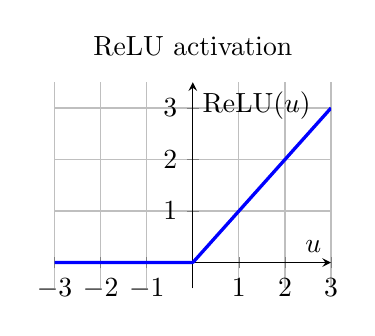
\begin{tikzpicture}
	\begin{axis}[
	width=0.42\textwidth,
	height=4.2cm,
	xmin=-3, xmax=3,
	ymin=-0.5, ymax=3.5,
	axis lines=middle,
	xlabel={$u$},
	ylabel={$\mathrm{ReLU}(u)$},
	samples=200,
	domain=-3:3,
	xtick={-3,-2,-1,0,1,2,3},
	ytick={0,1,2,3},
	grid=both,
	title={ReLU activation}
	]
	\addplot[very thick,blue] {max(0,x)};
	\end{axis}
	\end{tikzpicture}
	\hspace{0.5cm}
	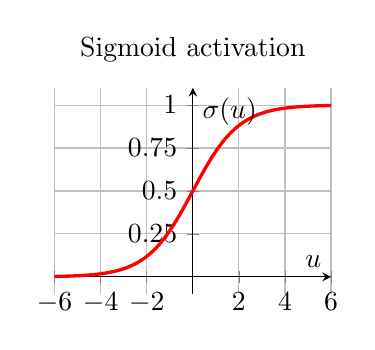
\begin{tikzpicture}
	\begin{axis}[
	width=0.42\textwidth,
	height=4.2cm,
	xmin=-6, xmax=6,
	ymin=-0.1, ymax=1.1,
	axis lines=middle,
	xlabel={$u$},
	ylabel={$\sigma(u)$},
	samples=200,
	domain=-6:6,
	xtick={-6,-4,-2,0,2,4,6},
	ytick={0,0.25,0.5,0.75,1},
	grid=both,
	title={Sigmoid activation}
	]
	\addplot[very thick,red] {1/(1+exp(-x))};
	\end{axis}
	\end{tikzpicture}
	\caption{ReLU and sigmoid activation functions used in the hidden and output layers, respectively.}
\end{figure}


The loss for a single sample is
\[
\mathcal{L} = \mathrm{BCE}(y,\hat y) + \frac{\lambda}{2}
\big(\|W^{[1]}\|_F^2 + \|W^{[2]}\|_2^2\big),
\]
where
\[
\mathrm{BCE}(y,\hat y) = -\Big(y\log\hat y + (1-y)\log(1-\hat y)\Big).
\]

\textbf{Tasks}
\begin{enumerate}
	\item[(a)] Compute the forward-pass values $z^{[1]}, a^{[1]}, z^{[2]}, \hat y = a^{[2]}$ and the final loss $\mathcal{L}$.
	\item[(b)] Compute $\dfrac{\partial\mathcal{L}}{\partial a^{[1]}}$.
	\item[(c)] Using backpropagation (including ReLU and L2 regularization), compute
	$\dfrac{\partial\mathcal{L}}{\partial W^{[1]}}$ and $\dfrac{\partial\mathcal{L}}{\partial x}$.
	\item[(d)] Suppose the first hidden neuron is a ``dying ReLU'', i.e. its pre-activation is always non-positive and therefore its ReLU output and gradient remain zero. Does the training algorithm still update that neuron’s weights? Explain using the gradient formulas.
\end{enumerate}

\subsection*{Solution}

\subsection{(a) Forward pass}

\paragraph{First layer pre-activation.}
\[
W^{[1]}x =
\begin{bmatrix}
0.5 & 1.0\\
0.5 & -2.0
\end{bmatrix}
\begin{bmatrix}
2\\
-1
\end{bmatrix}
=
\begin{bmatrix}
0.5\cdot 2 + 1.0\cdot(-1)\\
0.5\cdot 2 + (-2.0)\cdot(-1)
\end{bmatrix}
=
\begin{bmatrix}
0.0\\
3.0
\end{bmatrix}.
\]
Adding the bias:
\[
z^{[1]} = W^{[1]}x + b^{[1]} =
\begin{bmatrix}
0.0\\
3.0
\end{bmatrix}
+
\begin{bmatrix}
-1.5\\
0.5
\end{bmatrix}
=
\begin{bmatrix}
-1.5\\
3.5
\end{bmatrix}.
\]

\paragraph{Hidden activations (ReLU).}
\[
a^{[1]} = \mathrm{ReLU}(z^{[1]}) =
\begin{bmatrix}
\max(0,-1.5)\\
\max(0,3.5)
\end{bmatrix}
=
\begin{bmatrix}
0\\
3.5
\end{bmatrix}.
\]

\paragraph{Output pre-activation.}
\[
z^{[2]} = W^{[2]}a^{[1]} + b^{[2]}
= [1.0\;\;-1.0] \begin{bmatrix}0\\3.5\end{bmatrix} + 0
= 0 - 3.5 = -3.5.
\]

\paragraph{Output activation (sigmoid).}
\[
\hat y = \sigma(z^{[2]}) = \frac{1}{1+e^{-(-3.5)}}
= \frac{1}{1+e^{3.5}}
\approx 0.0293122.
\]

\paragraph{BCE loss (without regularization).}
Since $y=1$,
\[
\mathrm{BCE}(y,\hat y) = -\log(\hat y) \approx -\log(0.0293122) \approx 3.527.
\]

\paragraph{L2 regularization term.}
\[
\|W^{[1]}\|_F^2 =
0.5^2 + 1.0^2 + 0.5^2 + (-2.0)^2
= 0.25 + 1 + 0.25 + 4 = 5.5,
\]
\[
\|W^{[2]}\|_2^2 = 1.0^2 + (-1.0)^2 = 2.
\]
Total:
\[
\|W^{[1]}\|_F^2 + \|W^{[2]}\|_2^2 = 7.5.
\]
Thus
\[
\mathcal{L}_{\text{reg}}
= \frac{\lambda}{2}\cdot 7.5
= \frac{0.1}{2}\cdot 7.5 = 0.375.
\]

\paragraph{Total loss.}
\[
\mathcal{L} = \mathrm{BCE}(y,\hat y) + \mathcal{L}_{\text{reg}}
\approx 3.527 + 0.375 = 3.902.
\]

\noindent
\textbf{Summary of (a):}
\[
z^{[1]} =
\begin{bmatrix}
-1.5\\
3.5
\end{bmatrix},\quad
a^{[1]} =
\begin{bmatrix}
0\\
3.5
\end{bmatrix},\quad
z^{[2]} = -3.5,\quad
\hat y \approx 0.0293,\quad
\mathcal{L} \approx 3.902.
\]

\subsection{(b) Gradient with respect to $a^{[1]}$}

For BCE with a sigmoid output, for a single example:
\[
\frac{\partial\mathcal{L}}{\partial z^{[2]}} = \hat y - y.
\]
With $\hat y \approx 0.0293122$, $y=1$,
\[
\delta^{[2]} \equiv \frac{\partial\mathcal{L}}{\partial z^{[2]}}
= 0.0293122 - 1 \approx -0.9706878.
\]

The gradient w.r.t.\ the hidden activations is
\[
\frac{\partial\mathcal{L}}{\partial a^{[1]}}
= (W^{[2]})^\top \delta^{[2]}
=
\begin{bmatrix}
1.0\\
-1.0
\end{bmatrix}
(-0.9706878)
=
\begin{bmatrix}
-0.9706878\\
0.9706878
\end{bmatrix}.
\]

\[
\boxed{
	\frac{\partial\mathcal{L}}{\partial a^{[1]}}
	\approx
	\begin{bmatrix}
	-0.9707\\
	0.9707
	\end{bmatrix}
}
\]

\subsection{(c) Gradients w.r.t.\ $W^{[1]}$ and $x$}

\subsubsection*{ReLU backpropagation}

ReLU derivative:
\[
\mathrm{ReLU}'(u) =
\begin{cases}
1 & u > 0,\\
0 & u \le 0.
\end{cases}
\]
Here
\[
z^{[1]} =
\begin{bmatrix}
-1.5\\
3.5
\end{bmatrix}
\Rightarrow
\mathrm{ReLU}'(z^{[1]}) =
\begin{bmatrix}
0\\
1
\end{bmatrix}.
\]

Thus
\[
\delta^{[1]} \equiv
\frac{\partial\mathcal{L}}{\partial z^{[1]}}
=
\frac{\partial\mathcal{L}}{\partial a^{[1]}}
\odot \mathrm{ReLU}'(z^{[1]})
=
\begin{bmatrix}
-0.9706878\\
0.9706878
\end{bmatrix}
\odot
\begin{bmatrix}
0\\
1
\end{bmatrix}
=
\begin{bmatrix}
0\\
0.9706878
\end{bmatrix}.
\]

\subsubsection*{Gradient w.r.t.\ $W^{[1]}$}

Without regularization, for an affine layer $z^{[1]} = W^{[1]}x + b^{[1]}$:
\[
\frac{\partial\mathcal{L}}{\partial W^{[1]}} = \delta^{[1]} x^\top.
\]
Including L2 regularization:
\[
\frac{\partial\mathcal{L}}{\partial W^{[1]}}
= \delta^{[1]} x^\top + \lambda W^{[1]}.
\]

Compute $\delta^{[1]} x^\top$:
\[
x^\top = [\,2\;\; -1\,],
\]
\[
\delta^{[1]} x^\top =
\begin{bmatrix}
0\\
0.9706878
\end{bmatrix}
[\,2\;\; -1\,]
=
\begin{bmatrix}
0\cdot 2 & 0\cdot(-1)\\
0.9706878\cdot 2 & 0.9706878\cdot(-1)
\end{bmatrix}
=
\begin{bmatrix}
0 & 0\\
1.9413756 & -0.9706878
\end{bmatrix}.
\]

Regularization part:
\[
\lambda W^{[1]} = 0.1
\begin{bmatrix}
0.5 & 1.0\\
0.5 & -2.0
\end{bmatrix}
=
\begin{bmatrix}
0.05 & 0.10\\
0.05 & -0.20
\end{bmatrix}.
\]

Adding:
\[
\frac{\partial\mathcal{L}}{\partial W^{[1]}}
=
\begin{bmatrix}
0 & 0\\
1.9413756 & -0.9706878
\end{bmatrix}
+
\begin{bmatrix}
0.05 & 0.10\\
0.05 & -0.20
\end{bmatrix}
=
\begin{bmatrix}
0.05 & 0.10\\
1.9913756 & -1.1706878
\end{bmatrix}.
\]

\[
\boxed{
	\frac{\partial\mathcal{L}}{\partial W^{[1]}}
	\approx
	\begin{bmatrix}
	0.0500 & 0.1000\\
	1.9914 & -1.1707
	\end{bmatrix}
}
\]

In particular, for the $(1,1)$ element:
\[
\frac{\partial \mathcal{L}}{\partial W^{[1]}_{11}}
= 0 \;(\text{data term}) + 0.1 \cdot 0.5 = 0.05.
\]

The gradient w.r.t.\ the first-layer bias is
\[
\frac{\partial\mathcal{L}}{\partial b^{[1]}} = \delta^{[1]} =
\begin{bmatrix}
0\\
0.9706878
\end{bmatrix},
\]
with no regularization on $b^{[1]}$.

\subsubsection*{Gradient w.r.t.\ input $x$}

For $z^{[1]} = W^{[1]}x + b^{[1]}$,
\[
\frac{\partial\mathcal{L}}{\partial x} = (W^{[1]})^\top \delta^{[1]}.
\]

We have
\[
(W^{[1]})^\top =
\begin{bmatrix}
0.5 & 0.5\\
1.0 & -2.0
\end{bmatrix},\qquad
\delta^{[1]} =
\begin{bmatrix}
0\\
0.9706878
\end{bmatrix}.
\]

Therefore
\[
\frac{\partial\mathcal{L}}{\partial x} =
\begin{bmatrix}
0.5 & 0.5\\
1.0 & -2.0
\end{bmatrix}
\begin{bmatrix}
0\\
0.9706878
\end{bmatrix}
=
\begin{bmatrix}
0.5\cdot 0 + 0.5\cdot 0.9706878\\
1.0\cdot 0 + (-2.0)\cdot 0.9706878
\end{bmatrix}
=
\begin{bmatrix}
0.4853439\\
-1.9413756
\end{bmatrix}.
\]

\[
\boxed{
	\frac{\partial\mathcal{L}}{\partial x}
	\approx
	\begin{bmatrix}
	0.4853\\
	-1.9414
	\end{bmatrix}
}
\]

Regularization does not affect $\partial\mathcal{L}/\partial x$ because it depends only on the weights.

\subsection{(d) Dying ReLU and weight updates}

For a ReLU neuron $j$ in the hidden layer,
\[
a^{[1]}_j = \mathrm{ReLU}(z^{[1]}_j) = \max(0,z^{[1]}_j),
\]
\[
\frac{\partial a^{[1]}_j}{\partial z^{[1]}_j} =
\begin{cases}
1 & z^{[1]}_j > 0,\\
0 & z^{[1]}_j \le 0.
\end{cases}
\]

If neuron $j$ is ``dead'', then $z^{[1]}_j \le 0$ for all inputs.
Hence $\mathrm{ReLU}'(z^{[1]}_j)=0$, and
\[
\delta^{[1]}_j = \frac{\partial\mathcal{L}}{\partial z^{[1]}_j}
= \frac{\partial\mathcal{L}}{\partial a^{[1]}_j}
\cdot \frac{\partial a^{[1]}_j}{\partial z^{[1]}_j}
= \frac{\partial\mathcal{L}}{\partial a^{[1]}_j} \cdot 0 = 0.
\]

Therefore, for the weights from the input to neuron $j$,
\[
\frac{\partial\mathcal{L}}{\partial W^{[1]}_{j,:}}
= \delta^{[1]}_j x^\top + \lambda W^{[1]}_{j,:}
= 0\cdot x^\top + \lambda W^{[1]}_{j,:}
= \lambda W^{[1]}_{j,:}.
\]

The gradient with respect to its bias is
\[
\frac{\partial\mathcal{L}}{\partial b^{[1]}_j}
= \delta^{[1]}_j = 0,
\]
since biases are not regularized here.

\paragraph{Implications.}
\begin{itemize}
	\item If $\lambda = 0$ (no regularization), then
	\[
	\frac{\partial\mathcal{L}}{\partial W^{[1]}_{j,:}} = 0,
	\]
	so gradient descent will not update $W^{[1]}_{j,:}$ or $b^{[1]}_j$ at all: the neuron is permanently dead.
	
	\item With L2 regularization ($\lambda > 0$), the update for the weights of neuron $j$ becomes
	\[
	W^{[1]}_{j,:} \leftarrow W^{[1]}_{j,:} - \eta \frac{\partial\mathcal{L}}{\partial W^{[1]}_{j,:}}
	= W^{[1]}_{j,:} - \eta \lambda W^{[1]}_{j,:}
	= (1 - \eta\lambda) W^{[1]}_{j,:}.
	\]
	Thus the weights still change, but only due to regularization; they decay towards zero without receiving any learning signal from the data. The bias $b^{[1]}_j$ remains unchanged (its gradient is zero).
\end{itemize}

\paragraph{Answer.}
A dying ReLU neuron does not receive any data-driven gradient (its error term $\delta^{[1]}_j$ is zero). Without regularization, its weights and bias never change. With L2 regularization, its weights are updated only by the $\lambda W$ term, shrinking towards zero, while the neuron effectively stays inactive and does not ``revive''. Therefore, from the perspective of learning useful features, the algorithm does not meaningfully update that neuron once it has died.
\\
\\
\subsection{Network Diagram}
\begin{figure}[h!]
	\centering
	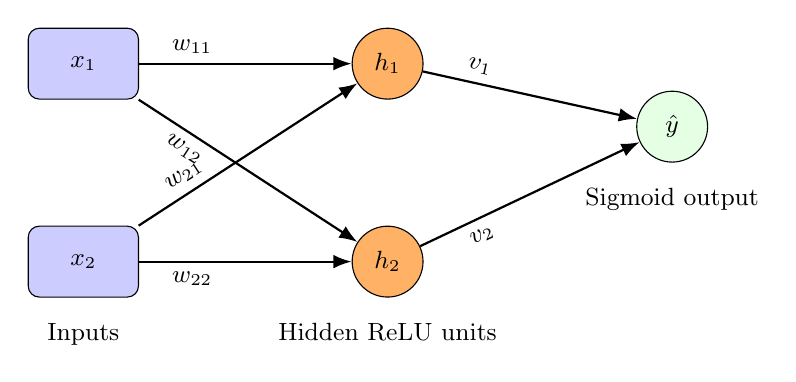
\begin{tikzpicture}[
	node distance=1.6cm and 2.2cm,
	box/.style={rectangle, draw=black, rounded corners,
		minimum width=1.4cm, minimum height=0.9cm,
		align=center},
	neuron/.style={circle, draw=black,
		minimum size=0.9cm,
		align=center},
	every node/.style={font=\small}
	]
	
	%--------------------
	% Input layer
	%--------------------
	\node[box, fill=blue!20]                     (x1) {$x_{1}$};
	\node[box, fill=blue!20, below=of x1]        (x2) {$x_{2}$};
	
	\node[below=0.2cm of x2] (inputlabel) {Inputs};
	
	%--------------------
	% Hidden layer
	%--------------------
	\node[neuron, fill=orange!60, right=2.7cm of x1] (h1) {$h_{1}$};
	\node[neuron, fill=orange!60, below=of h1]       (h2) {$h_{2}$};
	
	\node[below=0.2cm of h2] (hiddenlabel) {Hidden ReLU units};
	
	%--------------------
	% Output layer
	%--------------------
	\node[neuron, fill=green!10, right=2.7cm of h1, yshift=-0.8cm] (yhat) {$\hat{y}$};
	
	\node[below=0.2cm of yhat] (outputlabel) {Sigmoid output};
	
	%--------------------
	% Connections: input -> hidden
	%--------------------
	\draw[->, thick] (x1) -- node[above,sloped,near start] {$w_{11}$} (h1);
	\draw[->, thick] (x1) -- node[below,sloped,near start] {$w_{12}$} (h2);
	
	\draw[->, thick] (x2) -- node[above,sloped,near start] {$w_{21}$} (h1);
	\draw[->, thick] (x2) -- node[below,sloped,near start] {$w_{22}$} (h2);
	
	%--------------------
	% Connections: hidden -> output
	%--------------------
	\draw[->, thick] (h1) -- node[above,sloped,near start] {$v_{1}$} (yhat);
	\draw[->, thick] (h2) -- node[below,sloped,near start] {$v_{2}$} (yhat);
	
	\end{tikzpicture}
	\caption{Architecture of the network: 2 inputs, 2 hidden ReLU neurons, and 1 sigmoid output neuron.}
\end{figure}


\section{Question 2 (Problem Summary)}
	We study a deep MLP with $50$ layers using the Sigmoid activation.
We analyze:
\begin{itemize}
	\item[(a)] Why gradients vanish in such a deep Sigmoid network.
	\item[(b)] What happens when we instead use ReLU and Batch Normalization, and whether this allows very large learning rates without divergence; we also discuss how ReLU can still fail and what BN does to mitigate failure.
\end{itemize}

\subsection{(a) Vanishing Gradients in Deep Sigmoid Networks}

The Sigmoid function is
\[
\sigma(z)=\frac{1}{1+e^{-z}},
\qquad
\sigma'(z)=\sigma(z)(1-\sigma(z)).
\]
For all $z$,
\[
0 \le \sigma'(z)\le 0.25.
\]

When $z\gg 0$, $\sigma(z)\approx 1$ and $\sigma'(z)\approx 0$.
When $z\ll 0$, $\sigma(z)\approx 0$ and $\sigma'(z)\approx 0$.
The maximum derivative occurs at $z=0$, where $\sigma(0)=\tfrac12$ and
\[
\sigma'(0) = \tfrac12(1-\tfrac12)=\tfrac14.
\]

Consider backpropagation in a 50-layer network, with layers indexed
$l=1,\dots,50$.
For the loss $\mathcal{L}$ we have
\[
\frac{\partial\mathcal{L}}{\partial z^{[1]}}
=
\left(
\prod_{l=2}^{50}
W^{[l]T}
\operatorname{diag}(\sigma'(z^{[l]}))
\right)
\frac{\partial\mathcal{L}}{\partial z^{[50]}}.
\]

Taking norms, and assuming the weight matrices have moderate norms,
the dominant factor is the product of activation derivatives:
\[
\left\|
\frac{\partial\mathcal{L}}{\partial z^{[1]}}
\right\|
\;\lesssim\;
\Bigl(\max_z |\sigma'(z)|\Bigr)^{49}
\left\|
\frac{\partial\mathcal{L}}{\partial z^{[50]}}
\right\|
=
(0.25)^{49}
\left\|
\frac{\partial\mathcal{L}}{\partial z^{[50]}}
\right\|.
\]

Since
\[
(0.25)^{49} = 4^{-49} = 2^{-98} \approx 1.3\times 10^{-30},
\]
any reasonable gradient at the output layer is multiplied by an
astronomically small factor by the time it reaches the first layers.
In practice, many sigmoids are in saturated regions where
$\sigma'(z)\ll 0.25$, making this product even smaller.

Hence, gradients in early layers become essentially zero:
these layers learn extremely slowly or not at all.
This is the \emph{vanishing gradient problem}.

The value $0.25$ is crucial because it is the \emph{maximum} derivative
of the Sigmoid.  Since this maximum is already less than $1$, repeated
multiplication through many layers causes an exponential decay of
gradients with depth.
\\
\begin{itemize}
	\item Deep sigmoid MLP (50 layers) to visualize vanishing gradients.
	
\end{itemize}
\begin{figure}[h!]
	\centering
	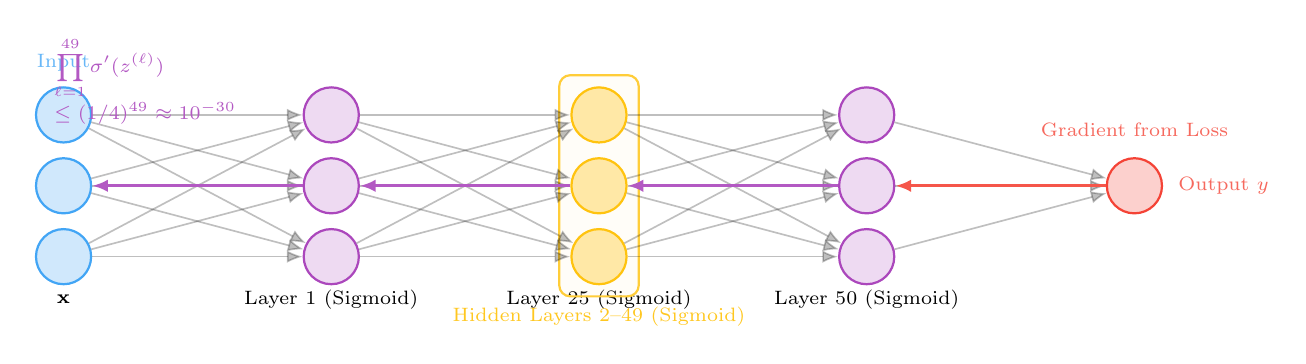
\begin{tikzpicture}[x=1.7cm,y=0.9cm]
	
	% --- INPUT LAYER ---
	\node[neuron, draw=inputblue, fill=inputblue!25] (x1) at (0, 1) {};
	\node[neuron, draw=inputblue, fill=inputblue!25] (x2) at (0, 0) {};
	\node[neuron, draw=inputblue, fill=inputblue!25] (x3) at (0,-1) {};
	
	\node[above=2pt of x1, text=inputblue!80] {\scriptsize Input};
	\node at (0,-1.6) {\scriptsize \(\mathbf{x}\)};
	
	% --- FIRST SIGMOID LAYER (L=1) ---
	\node[neuron, draw=sigmoidpurple, fill=sigmoidpurple!20] (h1a) at (2, 1) {};
	\node[neuron, draw=sigmoidpurple, fill=sigmoidpurple!20] (h1b) at (2, 0) {};
	\node[neuron, draw=sigmoidpurple, fill=sigmoidpurple!20] (h1c) at (2,-1) {};
	
	\node at (2,-1.6) {\scriptsize Layer 1 (Sigmoid)};
	
	% --- MIDDLE SIGMOID LAYERS (2--49) AS A BOX AROUND REPRESENTATIVE NEURONS ---
	\node[neuron, draw=hidden2, fill=hidden2!35] (m1) at (4,  1) {};
	\node[neuron, draw=hidden2, fill=hidden2!35] (m2) at (4,  0) {};
	\node[neuron, draw=hidden2, fill=hidden2!35] (m3) at (4, -1) {};
	\node at (4,-1.6) {\scriptsize Layer 25 (Sigmoid)};
	
	% Fit box around m1 and m3
	\node[layerbox,
	fill=hidden2!45,
	draw=hidden2!80,
	label={[hidden2!90]below:{\scriptsize Hidden Layers 2--49 (Sigmoid)}}]
	(MidBox) [fit=(m1) (m3)] {};
	
	% --- LAST SIGMOID LAYER (L=50) ---
	\node[neuron, draw=sigmoidpurple, fill=sigmoidpurple!20] (hL1) at (6,  1) {};
	\node[neuron, draw=sigmoidpurple, fill=sigmoidpurple!20] (hL2) at (6,  0) {};
	\node[neuron, draw=sigmoidpurple, fill=sigmoidpurple!20] (hL3) at (6, -1) {};
	
	\node at (6,-1.6) {\scriptsize Layer 50 (Sigmoid)};
	
	% --- OUTPUT LAYER ---
	\node[neuron, draw=outputred, fill=outputred!25] (y1) at (8,0) {};
	\node[right=2pt of y1, text=outputred!80] {\scriptsize Output \(y\)};
	
	% --- CONNECTIONS (FAINT) ---
	\foreach \i in {x1,x2,x3} {
		\foreach \j in {h1a,h1b,h1c} {
			\draw[conn,opacity=0.25] (\i) -- (\j);
		}
	}
	\foreach \i in {h1a,h1b,h1c} {
		\foreach \j in {m1,m2,m3} {
			\draw[conn,opacity=0.25] (\i) -- (\j);
		}
	}
	\foreach \i in {m1,m2,m3} {
		\foreach \j in {hL1,hL2,hL3} {
			\draw[conn,opacity=0.25] (\i) -- (\j);
		}
	}
	\foreach \i in {hL1,hL2,hL3} {
		\draw[conn,opacity=0.25] (\i) -- (y1);
	}
	
	% --- HIGHLIGHTED VANISHING GRADIENT PATH ---
	\draw[conn,very thick,draw=outputred!90] (y1) -- (hL2);
	\draw[conn,very thick,draw=sigmoidpurple!90] (hL2) -- (m2);
	\draw[conn,very thick,draw=sigmoidpurple!90] (m2) -- (h1b);
	\draw[conn,very thick,draw=sigmoidpurple!90] (h1b) -- (x2);
	
	\node[above=4pt of y1, align=center,text=outputred!80] 
	{\scriptsize Gradient from Loss};
	\node[above right=0.4cm and -0.5cm of x2, align=left,text=sigmoidpurple!90]
	{\scriptsize \(\displaystyle \prod_{\ell=1}^{49} \sigma'(z^{(\ell)})\)\\
		\scriptsize \(\le (1/4)^{49} \approx 10^{-30}\)};
	
	\end{tikzpicture}
	\caption{Deep sigmoid MLP: gradient from the output backward is multiplied
		by many small sigmoid derivatives (\(\le 1/4\)), leading to vanishing
		gradients in early layers.}
\end{figure}

\subsection{(b) ReLU, Large Learning Rates, and Batch Normalization}

Now we replace Sigmoid with ReLU:
\[
\mathrm{ReLU}(z) = \max(0,z),
\qquad
\mathrm{ReLU}'(z) =
\begin{cases}
1, & z>0,\\
0, & z\le 0.
\end{cases}
\]
We also use Batch Normalization (BN), which for pre-activations $z_i$
in a mini-batch computes
\[
\hat z_i = \frac{z_i - \mu_B}{\sqrt{\sigma_B^2 + \epsilon}},
\]
where $\mu_B$ and $\sigma_B^2$ are the batch mean and variance, and
$\epsilon$ is a small constant for numerical stability.

A student claims:
\emph{``Because we use Batch Normalization, we can choose very large
	learning rates, e.g.\ in the range $[10,20]$, and training will not
	diverge.''}

We analyze this claim and the roles of ReLU and BN.

\subsection*{(b1) Is the claim about very large learning rates correct?}

\textbf{No, this claim is not generally correct.}
Batch Normalization stabilizes the distribution of activations but does
not guarantee convergence for arbitrarily large learning rates:

\begin{itemize}
	\item BN normalizes activations to have approximately zero mean and
	unit variance per mini-batch, making the optimization landscape
	smoother and allowing somewhat larger learning rates than without BN.
	\item However, the \emph{parameters} can still change too abruptly if
	the learning rate is huge. Updates of size proportional to $10$
	or $20$ are typically far too large and can cause the loss to
	oscillate or diverge.
	\item BN controls the scale of $z$ within each batch, but it does not
	directly limit the magnitude of the weight updates.
\end{itemize}

Thus, while BN often allows training with a \emph{moderately} larger
learning rate, it does not make learning rates in $[10,20]$ safe in general.

\subsection*{(b2) Why can training still fail even with ReLU?}

Compared to Sigmoid, ReLU helps with vanishing gradients because
its derivative is $1$ whenever $z>0$.
Nevertheless, ReLU networks can still suffer from other failures:

\paragraph{Dying ReLU.}
If a neuron's pre-activation becomes negative for all training examples,
its output is always zero:
\[
a^{[l]} = \mathrm{ReLU}(z^{[l]}) = 0, \qquad
\mathrm{ReLU}'(z^{[l]}) = 0.
\]
Then the gradient through this neuron vanishes:
\[
\frac{\partial\mathcal{L}}{\partial W^{[l]}} = 0,
\]
and the neuron stops learning permanently (``dying ReLU'').
Large or poorly chosen updates (e.g.\ due to too large a learning rate)
can push many units into this inactive regime.

\paragraph{Exploding activations and gradients.}
If weights grow too large, the pre-activations $z^{[l]}$ and activations
$a^{[l]}$ can become very large.
This leads to very large gradients and unstable updates, causing
training to diverge.

\paragraph{Internal covariate shift.}
As earlier layers change, the distribution of activations feeding into
later layers keeps shifting. This can make optimization harder and
increase the risk that some units become mostly inactive or that
gradients become poorly scaled.

So even with ReLU, training can fail when the learning rate is too high
or the network becomes poorly conditioned.

\subsection*{(b3) Role of Batch Normalization}

Batch Normalization transforms pre-activations $z_i$ into
\[
\hat z_i = \frac{z_i - \mu_B}{\sqrt{\sigma_B^2 + \epsilon}},
\]
(and typically then applies a learned affine transformation).
This has several stabilizing effects:

\begin{itemize}
	\item \textbf{Keeps inputs to ReLU in a controlled range.} \\
	Since $\hat z_i$ has approximately zero mean and unit variance
	in each batch, roughly some fraction of values are positive and
	some negative. This reduces the chance that many ReLUs are
	always negative (dying) or always very large positive.
	\item \textbf{Reduces internal covariate shift.} \\
	As parameters in earlier layers change, BN re-normalizes each
	batch, so the distribution of activations seen by later layers
	changes less dramatically. This makes optimization more stable.
	\item \textbf{Stabilizes gradient magnitudes.} \\
	Controlling the variance of activations helps control the scale
	of backpropagated gradients, reducing exploding or vanishing
	gradients and making training less sensitive to initialization.
	\item \textbf{Allows moderately larger learning rates.} \\
	Because activations and gradients are better scaled, one can
	often use a somewhat larger learning rate than in an unnormalized
	network, and training can converge faster.
\end{itemize}

However, BN does \emph{not} guarantee that arbitrarily large learning
rates (such as $10$ or $20$) will work. Extremely large learning rates
can still cause large, unstable parameter updates that make training
diverge, even when BN is used.

\subsection*{(2) ReLU + Batch Normalization Block}

\begin{figure}[h!]
	\centering
	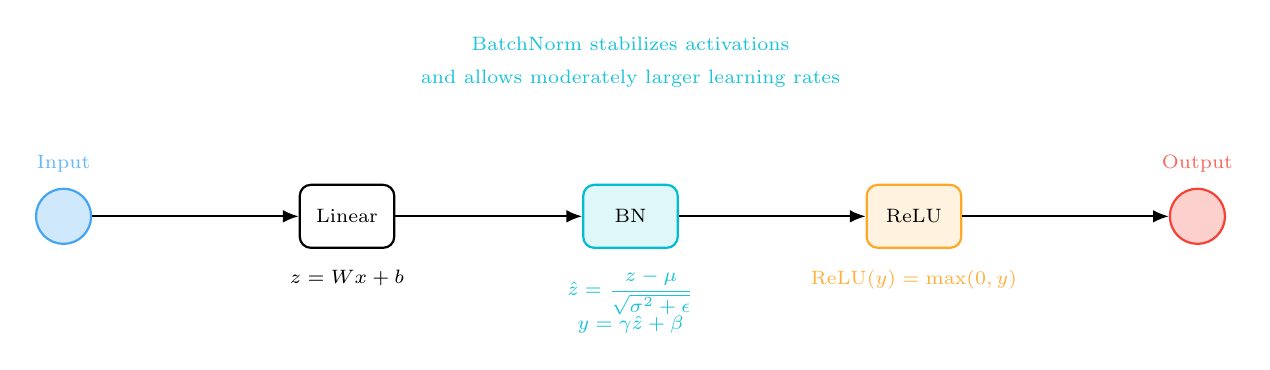
\begin{tikzpicture}[x=1.8cm,y=1.1cm]
	
	% Nodes
	\node[neuron,draw=inputblue,fill=inputblue!25] (x) at (0,0) {};
	\node[above=2pt of x,text=inputblue!80] {\scriptsize Input};
	
	\node[draw=black,rounded corners,thick,minimum width=1.2cm,minimum height=0.8cm] (W) at (2,0) {};
	\node at (2,0) {\scriptsize Linear};
	
	\node[draw=bncyan,rounded corners,thick,minimum width=1.2cm,minimum height=0.8cm,fill=bncyan!12] (BN) at (4,0) {};
	\node at (4,0) {\scriptsize BN};
	
	\node[draw=reluorange,rounded corners,thick,minimum width=1.2cm,minimum height=0.8cm,fill=reluorange!15] (ReLU) at (6,0) {};
	\node at (6,0) {\scriptsize ReLU};
	
	\node[neuron,draw=outputred,fill=outputred!25] (y) at (8,0) {};
	\node[above=2pt of y,text=outputred!80] {\scriptsize Output};
	
	% Connections
	\draw[conn] (x) -- (W);
	\draw[conn] (W) -- (BN);
	\draw[conn] (BN) -- (ReLU);
	\draw[conn] (ReLU) -- (y);
	
	% Annotations
	\node[below=4pt of W,align=center] {\scriptsize \(z = W x + b\)};
	\node[below=4pt of BN,align=center,text=bncyan!90]
	{\scriptsize \(\hat{z} = \dfrac{z-\mu}{\sqrt{\sigma^2+\epsilon}}\) \\
		\scriptsize \(y = \gamma \hat{z} + \beta\)};
	\node[below=4pt of ReLU,align=center,text=reluorange!90]
	{\scriptsize \(\mathrm{ReLU}(y) = \max(0,y)\)};
	
	\node[above=1.1cm of BN,align=center,text=bncyan!90]
	{\scriptsize BatchNorm stabilizes activations\\
		\scriptsize and allows moderately larger learning rates};
	
	\end{tikzpicture}
	\caption{A ReLU + BatchNorm block: BN normalizes activations before ReLU,
		stabilizing training, but does not make arbitrarily large learning
		rates always safe.}
\end{figure}


\paragraph{Conclusion.}
ReLU alleviates the classic vanishing gradient problem of Sigmoid, but
training can still fail due to dying ReLUs, exploding activations, and
poorly scaled updates. Batch Normalization stabilizes activations and
gradients, mitigates these issues, and allows moderately larger learning
rates, but it does not make training immune to divergence when the
learning rate is chosen excessively large.

\begin{figure}[h!]
	\centering
	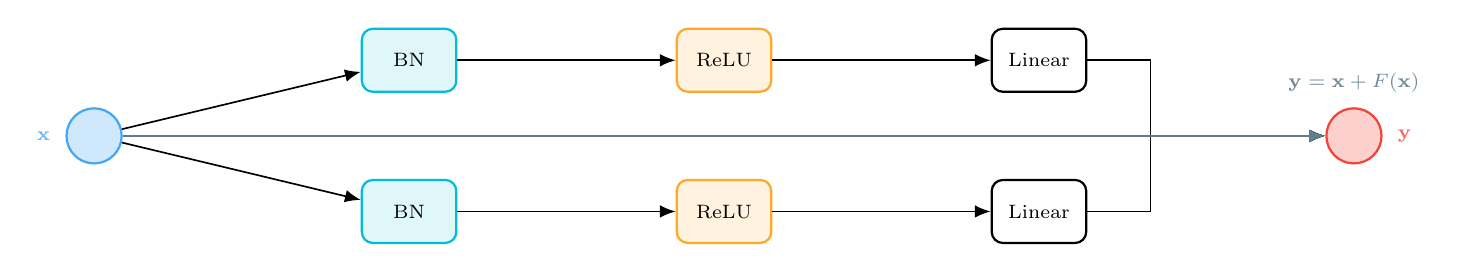
\begin{tikzpicture}[x=2cm,y=1.2cm]
	
	% Input
	\node[neuron,draw=inputblue,fill=inputblue!25] (x) at (0,0) {};
	\node[left=2pt of x,text=inputblue!80] {\scriptsize \(\mathbf{x}\)};
	
	% First BN+ReLU+Linear
	\node[draw=bncyan,rounded corners,thick,minimum width=1.2cm,minimum height=0.8cm,fill=bncyan!12] (BN1) at (2,0.8) {};
	\node at (BN1) {\scriptsize BN};
	\node[draw=reluorange,rounded corners,thick,minimum width=1.2cm,minimum height=0.8cm,fill=reluorange!15] (R1) at (4,0.8) {};
	\node at (R1) {\scriptsize ReLU};
	\node[draw=black,rounded corners,thick,minimum width=1.2cm,minimum height=0.8cm] (W1) at (6,0.8) {};
	\node at (W1) {\scriptsize Linear};
	
	% Second BN+ReLU+Linear
	\node[draw=bncyan,rounded corners,thick,minimum width=1.2cm,minimum height=0.8cm,fill=bncyan!12] (BN2) at (2,-0.8) {};
	\node at (BN2) {\scriptsize BN};
	\node[draw=reluorange,rounded corners,thick,minimum width=1.2cm,minimum height=0.8cm,fill=reluorange!15] (R2) at (4,-0.8) {};
	\node at (R2) {\scriptsize ReLU};
	\node[draw=black,rounded corners,thick,minimum width=1.2cm,minimum height=0.8cm] (W2) at (6,-0.8) {};
	\node at (W2) {\scriptsize Linear};
	
	% Output
	\node[neuron,draw=outputred,fill=outputred!25] (y) at (8,0) {};
	\node[right=2pt of y,text=outputred!80] {\scriptsize \(\mathbf{y}\)};
	
	% Main path connections
	\draw[conn] (x) -- (BN1);
	\draw[conn] (BN1) -- (R1);
	\draw[conn] (R1) -- (W1);
	\draw[conn] (W1.east) -- ++(0.4,0) |- (y);
	
	% Second path
	\draw[conn] (x) -- (BN2);
	\draw[conn] (BN2) -- (R2);
	\draw[conn] (R2) -- (W2);
	
	% Residual addition
	\draw[conn] (W2.east) -- ++(0.4,0) |- (y);
	
	% Skip connection (identity)
	\draw[conn,residualgray,thick] (x) -- ++(1.0,0) |- (y);
	
	% Label for residual
	\node[above=2pt of y,align=center,text=residualgray!90]
	{\scriptsize \(\mathbf{y} = \mathbf{x} + F(\mathbf{x})\)};
	
	\end{tikzpicture}
	\caption{A simple residual block: skip connections help gradients flow
		backward through many layers, mitigating vanishing gradients.}
\end{figure}

\newpage

\section{Question 3: Vectorized Implementation of Backpropagation and Adam}

\subsection{Task 1: Computing Gradients for Layer 1}
In this section, we implement the backward propagation for the first hidden layer (equipped with a ReLU activation function) using strictly vectorized operations in NumPy. 

The mathematical formulations for the gradients of the pre-activation $dZ^{[1]}$, weights $dW^{[1]}$, and biases $db^{[1]}$ for a mini-batch of size $m$ are as follows:

\begin{align}
dZ^{[1]} &= \left( W^{[2]T} dZ^{[2]} \right) \odot g'(Z^{[1]}) \\
dW^{[1]} &= \frac{1}{m} dZ^{[1]} X^T \\
db^{[1]} &= \frac{1}{m} \sum_{i=1}^{m} dZ^{[1](i)}
\end{align}

Where $\odot$ denotes the element-wise (Hadamard) product, and $g'(Z^{[1]})$ is the derivative of the ReLU function. The corresponding Python implementation is provided below:

\begin{lstlisting}[language=Python, caption={Vectorized Gradients Calculation for Layer 1}]
# 1. Compute dZ1 (Gradient of ReLU pre-activation)
# (A1 > 0) creates a boolean mask that acts as the exact derivative of the ReLU function.
dZ1 = np.dot(W2.T, dZ2) * (A1 > 0)

# 2. Compute dW1 and db1 explicitly
# The resulting dimensions will be (n_h, n_x) for dW1 and (n_h, 1) for db1.
dW1 = (1 / m) * np.dot(dZ1, X.T)

# The 'keepdims=True' argument is crucial to maintain the 2D shape (n_h, 1) 
# instead of flattening the array into a rank-1 array (n_h,).
db1 = (1 / m) * np.sum(dZ1, axis=1, keepdims=True)
\end{lstlisting}

\vspace{0.5cm}
\newpage
\subsection{Task 2: Adam Optimizer Updates for $W^{[1]}$}
In this task, we apply the Adam (Adaptive Moment Estimation) optimizer to update the weights of the first hidden layer ($W^{[1]}$). Adam combines the concepts of Momentum (tracking the gradient direction) and RMSProp (tracking the gradient magnitude) to adapt the learning rate individually for each parameter.

The mathematical formulation for the Adam update rule at timestep $t$ is defined as follows:

\begin{align}
m_t &= \beta_1 m_{t-1} + (1 - \beta_1) dW^{[1]} \quad &&\text{(Update First Moment)} \\
v_t &= \beta_2 v_{t-1} + (1 - \beta_2) \left(dW^{[1]}\right)^{\odot 2} \quad &&\text{(Update Second Moment)} \\
\hat{m}_t &= \frac{m_t}{1 - \beta_1^t} \quad &&\text{(Bias-Corrected First Moment)} \\
\hat{v}_t &= \frac{v_t}{1 - \beta_2^t} \quad &&\text{(Bias-Corrected Second Moment)} \\
W^{[1]}_{t+1} &= W^{[1]}_t - \frac{\eta}{\sqrt{\hat{v}_t} + \epsilon} \odot \hat{m}_t \quad &&\text{(Final Weight Update)}
\end{align}

Note that $\left(dW^{[1]}\right)^{\odot 2}$ indicates the element-wise square of the gradient. The default hyperparameters are $\beta_1 = 0.9$, $\beta_2 = 0.999$, $\eta = 0.01$ (learning rate), and $\epsilon = 10^{-8}$.


The corresponding vectorized Python implementation without any \texttt{for} loops is provided below:

\begin{lstlisting}[language=Python, caption={Adam Optimizer Update Rule for Layer 1 Weights}]
# Hyperparameters (defined by standard default values and the problem description)
beta1 = 0.9
beta2 = 0.999
lr = 0.01
epsilon = 1e-8

# 1. Update First Moment (Momentum)
# Tracks the moving average of the gradient.
m_t_new = beta1 * m_t + (1 - beta1) * dW1

# 2. Update Second Moment (RMSProp)
# Tracks the moving average of the squared gradient (element-wise).
v_t_new = beta2 * v_t + (1 - beta2) * np.square(dW1)

# 3. Bias Correction
# Corrects the initialization bias towards zero during the early timesteps.
m_t_hat = m_t_new / (1 - beta1 ** t)
v_t_hat = v_t_new / (1 - beta2 ** t)

# 4. Final Weight Update
# Updates the weights using the adaptive learning rate.
W1_updated = W1 - lr * (m_t_hat / (np.sqrt(v_t_hat) + epsilon))
\end{lstlisting}

\vspace{0.5cm}

\newpage
\subsection{Task 3: Analytical Question on \texttt{keepdims} and Broadcasting}

\textbf{1. Why is \texttt{keepdims=True} required when computing $db^{[1]}$?} \\
The gradient matrix $dZ^{[1]}$ has dimensions $(n\_h, m)$. When we apply \texttt{np.sum(dZ1, axis=1)} to sum across the mini-batch examples (the columns), NumPy inherently collapses the dimension over which the sum is computed. Without setting \texttt{keepdims=True}, the output collapses into a 1D rank-1 array with shape $(n\_h,)$, which is neither a row vector nor a column vector. By explicitly using \texttt{keepdims=True}, NumPy retains the collapsed dimension as a size of 1, resulting in a proper 2D column vector of shape $(n\_h, 1)$. This strictly matches the required mathematical dimensions for the bias vector $b^{[1]}$.

\vspace{0.3cm}
\textbf{2. What happens to Python Broadcasting in the next iteration if omitted?} \\
If \texttt{keepdims} is omitted and $db^{[1]}$ (and subsequently the updated $b^{[1]}$) becomes a rank-1 array of shape $(n\_h,)$, a critical alignment issue will occur during the forward propagation of the next training iteration. The equation for the linear transformation is $Z^{[1]} = W^{[1]} X + b^{[1]}$. 

The matrix multiplication $W^{[1]} X$ yields a matrix of shape $(n\_h, m)$. According to NumPy's broadcasting rules, which align trailing dimensions from right to left, an array of shape $(n\_h,)$ is interpreted as a row vector $(1, n\_h)$. NumPy will inappropriately attempt to broadcast this row vector across the $(n\_h, m)$ matrix. 
\begin{itemize}
	\item If $m \neq n\_h$ (which is typical), the code will instantly crash with a \texttt{ValueError: operands could not be broadcast together}.
	\item If $m = n\_h$ (an edge case), the program will not crash, but the biases will be added column-wise instead of row-wise, leading to a silent and catastrophic mathematical corruption that prevents the network from converging.
\end{itemize}

\newpage
\subsection{Complete Python Implementation}
For clarity and grading purposes, the complete, vectorized implementation for calculating the gradients and applying the Adam optimizer updates without any \texttt{for} loops is provided below:

\begin{lstlisting}[language=Python, caption={Complete Vectorized Backward Propagation and Adam Update}]
def backward_and_adam_update(X, A1, W2, dZ2, W1, b1, m, t, m_t, v_t):
"""
Computes gradients for the first layer and updates W1 using the Adam Optimizer.
"""
# --- Task 1: Compute Gradients for Layer 1 ---

# 1. Compute dZ1 (Gradient of ReLU pre-activation)
# (A1 > 0) creates a boolean mask that acts as the exact derivative of ReLU.
dZ1 = np.dot(W2.T, dZ2) * (A1 > 0)

# 2. Compute dW1 and db1 explicitly
# Resulting shapes: dW1 -> (n_h, n_x), db1 -> (n_h, 1)
dW1 = (1 / m) * np.dot(dZ1, X.T)
db1 = (1 / m) * np.sum(dZ1, axis=1, keepdims=True)

# --- Task 2: Adam Optimizer Updates for W1 ---

# Hyperparameters (typical default values)
beta1 = 0.9
beta2 = 0.999
lr = 0.01
epsilon = 1e-8

# 1. Update First Moment (Momentum)
m_t_new = beta1 * m_t + (1 - beta1) * dW1

# 2. Update Second Moment (RMSProp)
v_t_new = beta2 * v_t + (1 - beta2) * np.square(dW1)

# 3. Bias Correction for First and Second Moments
m_t_hat = m_t_new / (1 - beta1 ** t)
v_t_hat = v_t_new / (1 - beta2 ** t)

# 4. Final Weight Update
W1_updated = W1 - lr * (m_t_hat / (np.sqrt(v_t_hat) + epsilon))

return W1_updated, m_t_new, v_t_new
\end{lstlisting}


\section{Question 4: Theoretical Analysis of Dropout and Scaling}

\textbf{Setup:}
Consider a hidden neuron with a pre-activation value $a = 10$. The Dropout mechanism is applied with a drop probability $p = 0.5$, effectively acting as a Bernoulli mask during the training phase.

\subsection{(a) Statistical Expectation in the Training Phase}

During training, the neuron's output is a stochastic variable, $y_{train}$, which depends on the dropout state. The probability distribution is defined as:
\[
y_{train} = 
\begin{cases} 
a & \text{with probability } (1-p) = 0.5 \\
0 & \text{with probability } p = 0.5 
\end{cases}
\]

To find the average behavior of this neuron during the forward pass, we calculate its expected value:
\[
\mathbb{E}[y_{train}] = \sum y \cdot P(y) = (a \times 0.5) + (0 \times 0.5)
\]
\[
\mathbb{E}[y_{train}] = 10 \times 0.5 = 5
\]

\textbf{Result:} The mean activation level that the subsequent layers learn to represent during training is $\boxed{5}$.

\subsection{(b) Inference Discrepancy and Calibration Strategies}

At test time (Inference), the stochastic Dropout is deactivated to ensure deterministic outputs. Thus, the neuron consistently yields $y_{test} = a = 10$.

\textbf{The Mismatch:}
Comparing the two phases, we observe that $y_{test} = 10$ while $\mathbb{E}[y_{train}] = 5$. This factor-of-two difference ($y_{test} = \frac{1}{1-p} \mathbb{E}[y_{train}]$) leads to a magnitude shift in the input distribution of the following layers, which can significantly degrade model performance.

\subsubsection*{Mathematical Resolutions:}
To maintain consistency between training and inference, we can employ one of the following two scaling techniques:

\vspace{0.3cm}
\noindent \textbf{Option 1: Inverted Dropout Strategy (Active Learning)} \\
This is the modern approach where we compensate for the dropped energy \textit{during the training phase}. We scale the active neurons by a factor of $\frac{1}{1-p}$:
\[
\hat{y}_{train} = \frac{y_{train}}{1-p} = \frac{y_{train}}{0.5} = 2 \cdot y_{train}
\]
In this case, the new expectation becomes $\mathbb{E}[\hat{y}_{train}] = 10$, which aligns perfectly with the test-time output $y_{test} = 10$ without requiring any modifications during inference.

\vspace{0.3cm}
\noindent \textbf{Option 2: Post-Training Weight Scaling (Classic Approach)} \\
Alternatively, we can keep the training phase as is and apply a correction \textit{during inference}. We scale the weights or the activation by the keep probability $(1-p)$:
\[
\hat{y}_{test} = a \times (1-p) = 10 \times 0.5 = 5
\]
By reducing the inference-time activation to 5, we match the expected signal level that the network was optimized for during the training process.


\section{Question 5: Exoplanet Habitable Zone (Coding Challenge)}

\subsection{Phase 1: Proving the Deadlock of Linear Models}

In this phase, we evaluate the performance of a simple linear classifier—specifically Logistic Regression—on the "Habitable Zone" dataset. The dataset follows a non-linear concentric circle structure, where habitable planets (Class 1) are located in an inner ring, surrounded by uninhabitable planets (Class 0).

\textbf{Model Accuracy:} \\
Upon training the Logistic Regression model on the training set and evaluating its performance on the test data, the achieved accuracy was approximately \textbf{41.67\%}. This result is significantly lower than a standard threshold and reflects the model's inability to distinguish between the two classes.

\textbf{Mathematical and Geometric Analysis of Failure:} \\
The failure of this model is rooted in the concept of \textbf{Linear Separability}. A linear classifier (such as Logistic Regression or a single-layer Perceptron) is mathematically constrained to producing a straight decision boundary (a hyperplane) in the feature space. 

As visualized in Figure \ref{fig:phase1_linear_boundary}, the classes in this dataset are distributed in a way that no single straight line can isolate the inner circle from the outer ring. Consequently, the linear boundary intersects both classes regardless of its orientation, leading to high classification error and proving that linear models are insufficient for capturing radial or non-linear patterns. 

\begin{figure}[H]
	\centering
	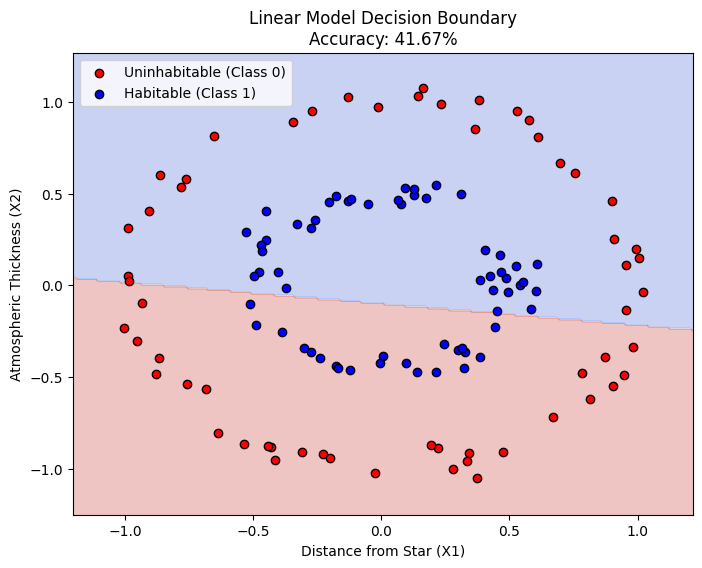
\includegraphics[width=0.75\textwidth]{1.png}
	\caption{Decision boundary of the linear Logistic Regression model. The straight boundary illustrates the model's failure to adapt to the circular geometry of the data.}
	\label{fig:phase1_linear_boundary}
\end{figure}

\subsubsection*{Python Implementation}
The following code was implemented in Google Colab to generate the dataset, train the linear model, and visualize the resulting decision boundary:

\begin{lstlisting}[language=Python, caption=Logistic Regression Implementation for Phase 1]
import numpy as np
import matplotlib.pyplot as plt
from sklearn.datasets import make_circles
from sklearn.model_selection import train_test_split
from sklearn.linear_model import LogisticRegression
from sklearn.metrics import accuracy_score

# 1. Generate the "Habitable Zone" dataset
X, y = make_circles(n_samples=600, noise=0.05, factor=0.5, random_state=42)
X_train, X_test, y_train, y_test = train_test_split(X, y, test_size=0.2, random_state=42)

# 2. Train a Simple Linear Classifier (Logistic Regression without hidden layers)
linear_model = LogisticRegression()
linear_model.fit(X_train, y_train)

# 3. Calculate Accuracy on Test Data
y_pred = linear_model.predict(X_test)
accuracy = accuracy_score(y_test, y_pred)
print(f"Test Accuracy: {accuracy * 100:.2f}%")

# 4. Plotting the Decision Boundary
def plot_decision_boundary(model, X, y, title):
# Set min and max values and give it some padding
x_min, x_max = X[:, 0].min() - 0.2, X[:, 0].max() + 0.2
y_min, y_max = X[:, 1].min() - 0.2, X[:, 1].max() + 0.2
h = 0.01 # Step size in the mesh

# Generate a grid of points with distance h between them
xx, yy = np.meshgrid(np.arange(x_min, x_max, h), np.arange(y_min, y_max, h))

# Predict the function value for the whole grid
Z = model.predict(np.c_[xx.ravel(), yy.ravel()])
Z = Z.reshape(xx.shape)

# Plot the contour and training examples
plt.figure(figsize=(8, 6))
plt.contourf(xx, yy, Z, alpha=0.3, cmap=plt.cm.coolwarm)
plt.scatter(X[y==0, 0], X[y==0, 1], color='red', label='Uninhabitable (Class 0)', edgecolors='k')
plt.scatter(X[y==1, 0], X[y==1, 1], color='blue', label='Habitable (Class 1)', edgecolors='k')

plt.xlabel('Distance from Star (X1)')
plt.ylabel('Atmospheric Thickness (X2)')
plt.title(title)
plt.legend()
plt.show()

plot_decision_boundary(linear_model, X_test, y_test, f"Linear Model Decision Boundary\nAccuracy: {accuracy * 100:.2f}%")
\end{lstlisting}


\subsection{Phase 2: The Minimalist Architect Challenge}

In this phase, we leverage the Universal Approximation Theorem to classify the concentric dataset using an MLP with a single hidden layer and ReLU activation functions. The objective is to find the absolute minimum number of hidden neurons required to achieve an accuracy exceeding 95\% by successfully enclosing the inner class (habitable zone).

\textbf{Geometric Interpretation of ReLU Neurons:} \\
Answering the core geometric question: \textit{What is the geometric equivalent of a ReLU neuron in the input space?} \\
Each neuron in a hidden layer with a ReLU activation function effectively draws a straight line (a hyperplane) that divides the 2D input space into two half-spaces: one where the neuron is active ($>0$) and one where it is inactive ($=0$). To successfully isolate the inner circular class (Class 1) from the outer ring (Class 0), the network must intersect these half-spaces to form a \textbf{closed convex polygon} around the inner planets.

Based on the empirical decision boundaries shown in Figure \ref{fig:phase2_neurons}, we can mathematically explain why certain architectures fail or succeed:
\begin{itemize}
	\item \textbf{1 Neuron (Accuracy 41.67\%):} Draws only a single line. It leaves the space completely open, acting just like a linear model, and therefore \textbf{never} solves the problem.
	\item \textbf{2 Neurons (Accuracy 49.17\%):} Can draw two lines, creating an open region (such as a 'V' shape or a parallel strip). It is geometrically impossible to fully enclose a central region using only two lines, meaning it will \textbf{never} separate the classes.
	\item \textbf{3 Neurons (Accuracy 71.67\%):} Three intersecting lines can theoretically form a closed triangle. However, as seen in our experiment, the optimization often settles into a local minimum (forming an open band) rather than a perfect triangle.
	\item \textbf{4 Neurons (Accuracy 100.00\%):} Provides four lines, which easily form a closed quadrilateral (a diamond-like bounding box). The network successfully constructs a perfect trap around the habitable zone.
\end{itemize}

\textbf{Conclusion:} While 3 neurons is the theoretical absolute minimum to form a closed shape, \textbf{4 neurons} is the minimalist architecture required in practice to successfully and consistently separate this dataset with $>95\%$ accuracy.

\begin{figure}[H]
	\centering
	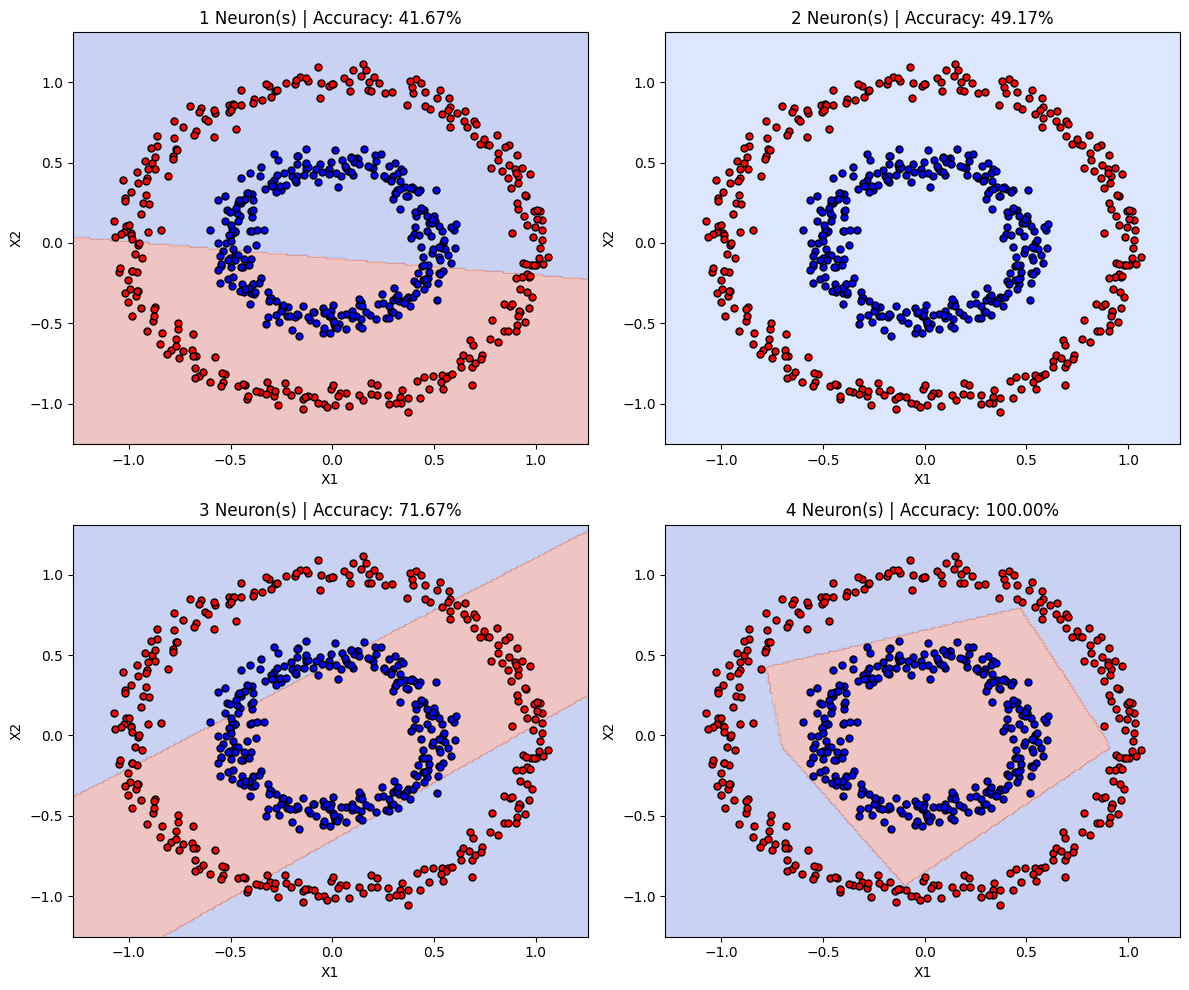
\includegraphics[width=0.95\textwidth]{2.png}
	\caption{Geometric analysis of the decision boundary formed by an MLP with a single hidden layer containing 1, 2, 3, and 4 ReLU neurons. A closed polygon (achieved here with 4 neurons) is necessary to enclose the inner class.}
	\label{fig:phase2_neurons}
\end{figure}

\subsubsection*{Python Implementation}
The following Colab script demonstrates the iterative training of the minimal MLP models using the \texttt{lbfgs} solver, which is highly optimized for small datasets:

\begin{lstlisting}[language=Python, caption=MLP Minimum Architecture Search]
import numpy as np
import matplotlib.pyplot as plt
from sklearn.datasets import make_circles
from sklearn.model_selection import train_test_split
from sklearn.neural_network import MLPClassifier
from sklearn.metrics import accuracy_score

# 1. Generate the dataset
X, y = make_circles(n_samples=600, noise=0.05, factor=0.5, random_state=42)
X_train, X_test, y_train, y_test = train_test_split(X, y, test_size=0.2, random_state=42)

# List of neurons to test
neurons_list = [1, 2, 3, 4]

plt.figure(figsize=(12, 10))

for i, n in enumerate(neurons_list):
# 2. Build and train MLP with 'n' neurons in the single hidden layer
# We use 'lbfgs' solver which is highly efficient for small datasets/architectures
mlp = MLPClassifier(hidden_layer_sizes=(n,), activation='relu', solver='lbfgs', max_iter=2000, random_state=42)
mlp.fit(X_train, y_train)

# 3. Predict and calculate accuracy
y_pred = mlp.predict(X_test)
accuracy = accuracy_score(y_test, y_pred)
print(f"Number of Neurons: {n} -> Test Accuracy: {accuracy * 100:.2f}%")

# 4. Plot Decision Boundary
plt.subplot(2, 2, i + 1)
x_min, x_max = X[:, 0].min() - 0.2, X[:, 0].max() + 0.2
y_min, y_max = X[:, 1].min() - 0.2, X[:, 1].max() + 0.2
xx, yy = np.meshgrid(np.arange(x_min, x_max, 0.01), np.arange(y_min, y_max, 0.01))

Z = mlp.predict(np.c_[xx.ravel(), yy.ravel()]).reshape(xx.shape)

plt.contourf(xx, yy, Z, alpha=0.3, cmap=plt.cm.coolwarm)
plt.scatter(X[y==0, 0], X[y==0, 1], color='red', label='Class 0', edgecolors='k', s=25)
plt.scatter(X[y==1, 0], X[y==1, 1], color='blue', label='Class 1', edgecolors='k', s=25)

plt.title(f"{n} Neuron(s) | Accuracy: {accuracy * 100:.2f}%")
plt.xlabel('X1')
plt.ylabel('X2')

plt.tight_layout()
plt.show()
\end{lstlisting}

\subsection{Phase 3: The Activation Trap (Vanishing Gradients)}

In this final phase, we investigate the impact of activation functions on the convergence speed of a relatively deep architecture (3 hidden layers, 10 neurons each) trained with a learning rate of $0.01$.

\textbf{Loss Curve Observation:} \\
As illustrated in Figure \ref{fig:phase3_loss}, there is a stark contrast in the learning dynamics of the two networks. The loss curve for the ReLU-activated network (blue line) decreases smoothly and rapidly towards zero, indicating successful and robust convergence. Conversely, the loss curve for the Sigmoid-activated network (red line) remains entirely flat and stagnant from the very first epochs, demonstrating a complete failure to optimize the weights.

\textbf{Identification of the Phenomenon:} \\
This catastrophic failure in the Sigmoid-based network is a textbook manifestation of the \textbf{Vanishing Gradient Problem}. As the network depth increases, the early hidden layers fail to receive meaningful gradient updates, effectively trapping the network in its initial state and halting the learning process.

\textbf{Mathematical Justification via Derivatives:} \\
The root cause of this phenomenon lies in the mathematical properties of the activation functions' derivatives applied during backpropagation via the Chain Rule:
\begin{itemize}
	\item \textbf{Sigmoid Activation:} The derivative of the sigmoid function, $\sigma'(z) = \sigma(z)(1 - \sigma(z))$, has an absolute maximum value of $0.25$ (at $z=0$). During backpropagation through 3 hidden layers, the error gradient from the output layer is continuously multiplied by these fractional derivatives. The compound effect is at best $(0.25)^3 \approx 0.015$, and practically much closer to zero. This exponential decay causes the gradients to "vanish" before they can update the weights of the initial layers.
	\item \textbf{ReLU Activation:} The derivative of the Rectified Linear Unit is exactly $1$ for all positive inputs ($z > 0$). This constant gradient ensures that active neurons backpropagate the error signal without any attenuation (repeated multiplication by 1). Consequently, early layers receive strong, unaltered gradients, allowing the deep network to update its weights and converge rapidly.
\end{itemize}

\begin{figure}[H]
	\centering
	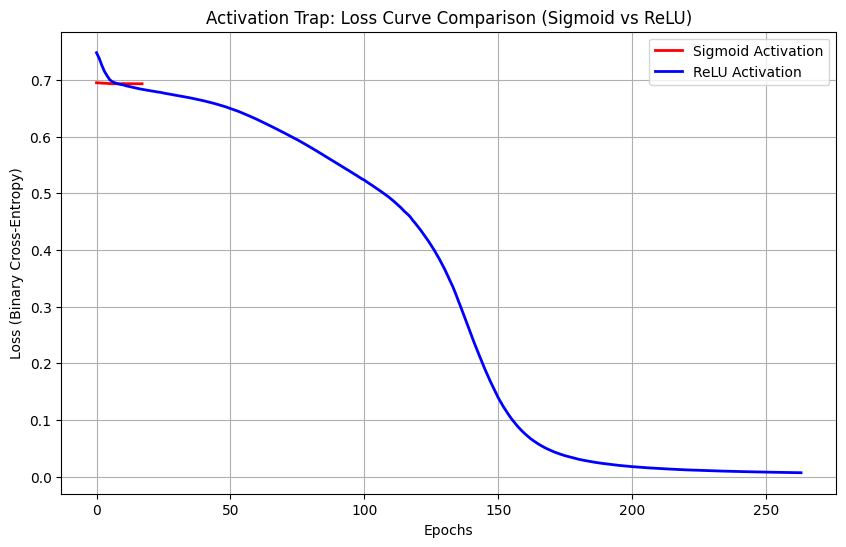
\includegraphics[width=0.85\textwidth]{3.png}
	\caption{Loss curve comparison between Sigmoid and ReLU activations. The flat red line practically demonstrates the Vanishing Gradient problem in deep Sigmoid networks, whereas the ReLU network converges successfully.}
	\label{fig:phase3_loss}
\end{figure}

\subsubsection*{Python Implementation}
The execution and plotting of the loss curves were implemented as follows:

\begin{lstlisting}[language=Python, caption=Comparing Convergence: Sigmoid vs ReLU]
import numpy as np
import matplotlib.pyplot as plt
from sklearn.datasets import make_circles
from sklearn.model_selection import train_test_split
from sklearn.neural_network import MLPClassifier

# 1. Generate the dataset
X, y = make_circles(n_samples=600, noise=0.05, factor=0.5, random_state=42)
X_train, X_test, y_train, y_test = train_test_split(X, y, test_size=0.2, random_state=42)

# 2. Common hyperparameters (3 hidden layers with 10 neurons each, LR = 0.01)
common_params = {
'hidden_layer_sizes': (10, 10, 10),
'learning_rate_init': 0.01,
'solver': 'sgd',  # SGD perfectly illustrates the Vanishing Gradient problem
'max_iter': 1000,
'random_state': 42
}

# 3. Train Model 1: Sigmoid (Logistic)
mlp_sigmoid = MLPClassifier(activation='logistic', **common_params)
mlp_sigmoid.fit(X_train, y_train)

# 4. Train Model 2: ReLU
mlp_relu = MLPClassifier(activation='relu', **common_params)
mlp_relu.fit(X_train, y_train)

# 5. Plot the Loss Curves
plt.figure(figsize=(10, 6))
plt.plot(mlp_sigmoid.loss_curve_, label='Sigmoid Activation', color='red', linewidth=2)
plt.plot(mlp_relu.loss_curve_, label='ReLU Activation', color='blue', linewidth=2)

plt.title('Activation Trap: Loss Curve Comparison (Sigmoid vs ReLU)')
plt.xlabel('Epochs')
plt.ylabel('Loss (Binary Cross-Entropy)')
plt.legend()
plt.grid(True)
plt.show()

# Print accuracies for reference
print(f"Sigmoid Test Accuracy: {mlp_sigmoid.score(X_test, y_test)*100:.2f}%")
print(f"ReLU Test Accuracy: {mlp_relu.score(X_test, y_test)*100:.2f}%")
\end{lstlisting}



\end{document}
